% !TeX program = pdfLaTeX
\documentclass[smallextended]{svjour3}       % onecolumn (second format)
%\documentclass[twocolumn]{svjour3}          % twocolumn
%
\smartqed  % flush right qed marks, e.g. at end of proof
%
\usepackage{amsmath}
\usepackage{graphicx}
\usepackage[utf8]{inputenc}

\usepackage[hyphens]{url} % not crucial - just used below for the URL
\usepackage{hyperref}
\providecommand{\tightlist}{%
  \setlength{\itemsep}{0pt}\setlength{\parskip}{0pt}}

%
% \usepackage{mathptmx}      % use Times fonts if available on your TeX system
%
% insert here the call for the packages your document requires
%\usepackage{latexsym}
% etc.
%
% please place your own definitions here and don't use \def but
% \newcommand{}{}
%
% Insert the name of "your journal" with
% \journalname{myjournal}
%

%% load any required packages here
\usepackage{caption}
\usepackage{ltablex}
\usepackage{pdflscape}
\usepackage{multirow}
\usepackage{placeins}




\begin{document}

\title{Open source landscape ecology tools \thanks{Grants or other notes about the article that should go on the front
page should be placed here. General acknowledgments should be placed at the
end of the article.} }



\author{  Maximillian H.K. Hesselbarth \and  Jakub Nowosad \and  Author 3 \and  \ldots{} \and  }


\institute{
        Maximillian H.K. Hesselbarth \at
     Department of Ecosystem Modelling, University of Goettingen, Buesgenweg 4, 37077 Goettingen, Germany \\
     \email{\href{mailto:mhk.hesselbarth@gmail.com}{\nolinkurl{mhk.hesselbarth@gmail.com}}}  %  \\
%             \emph{Present address:} of F. Author  %  if needed
    \and
        Jakub Nowosad \at
     Institute of Geoecology and Geoinformation, Adam Mickiewicz University, Krygowskiego 10, 61-680 Poznan, Poland \\
     \email{\href{mailto:nowosad.jakub@gmail.com}{\nolinkurl{nowosad.jakub@gmail.com}}}  %  \\
%             \emph{Present address:} of F. Author  %  if needed
    \and
        Author 3 \at
     Adress author 3 \\
     \email{E-Mail author 3}  %  \\
%             \emph{Present address:} of F. Author  %  if needed
    \and
        \ldots{} \at
     \ldots{} \\
     \email{\ldots{}}  %  \\
%             \emph{Present address:} of F. Author  %  if needed
    \and
    }

\date{Received: date / Accepted: date}
% The correct dates will be entered by the editor


\maketitle

\begin{abstract}
max. (200 words) Abstract Abstract Abstract Abstract Abstract Abstract Abstract Abstract Abstract Abstract Abstract Abstract Abstract Abstract Abstract Abstract Abstract Abstract Abstract Abstract Abstract Abstract Abstract Abstract Abstract Abstract Abstract Abstract Abstract Abstract Abstract Abstract Abstract Abstract Abstract Abstract Abstract Abstract Abstract Abstract Abstract Abstract Abstract Abstract Abstract Abstract Abstract Abstract Abstract Abstract Abstract Abstract Abstract Abstract Abstract Abstract Abstract Abstract Abstract Abstract Abstract Abstract Abstract Abstract Abstract Abstract Abstract Abstract Abstract Abstract Abstract Abstract Abstract Abstract Abstract Abstract Abstract Abstract Abstract Abstract Abstract Abstract Abstract Abstract Abstract Abstract Abstract Abstract Abstract Abstract Abstract Abstract Abstract Abstract Abstract Abstract Abstract Abstract Abstract Abstract
\\
\keywords{
        keyword 1 \and
        keyword 2 \and
        keyword 3 \and
        keyword 4 \and
        \ldots{} \and
    }


\end{abstract}


\def\spacingset#1{\renewcommand{\baselinestretch}%
{#1}\small\normalsize} \spacingset{1}


\hypertarget{sec:intro}{%
\section{Introduction}\label{sec:intro}}

\hypertarget{sec:landscape_ecology}{%
\subsection{A short introduction to landscape ecology}\label{sec:landscape_ecology}}

Landscape ecology focuses on how ecological processes are influenced and modified by the heterogeneous landscapes they occur in and simultaneously how the ecological processes themselves influence the landscapes \cite{Turner1989,Turner2005,With2019}.
In this context, landscape ecology considers, besides others, i) spatial and temporal dynamics of heterogeneous landscapes, ii) interactions, fluxes and exchange within these landscapes, iii) how the landscapes influence ecological processes (and vice versa) and lastly iv) how to manage these heterogeneous landscapes \cite{Risser1984,Turner1989}.

While human activities have altered the landscapes for millenniums \cite{Ellis2011,Ellis2015}, in the past centuries the effects of humans on landscapes have increased to an unknown high, known as the the Anthropocene \cite{Crutzen2002}.
Today, almost all landscapes are directly or indirectly influenced by human activities \cite{Vitousek1997}.
Thus, understanding the complex interactions between landscapes and ecological processes becomes increasingly important \cite{With2019}.

Because landscapes are defined as mosaics of different land covers, ecosystems, habitat types, or land uses \cite{Forman1986,Forman1995,Wiens1995}, spatial context is important and ecological processes will vary spatially \cite{With2019}.
to this, the importance of scale was already raised decades ago \cite{Wiens1989,Levin1992,Jelinski1996} and is still of relevance until today \cite{Simova2012,Estes2018}.
Thus, in contrast to many other sub-disciplines of ecology, landscape ecology emphasizes especially spatial patterns to a high degree \cite{Risser1984}.
Consequently, the field of landscape ecology relies on software to preprocess, modify, model, analyze and visualize spatial data.

\hypertarget{sec:open_source}{%
\subsection{Open-source software and R}\label{sec:open_source}}

Software to manage and analyze data becomes increasingly important in modern scientific research \cite{Wilson2014} and many scientific studies would not have been possible without open-source software \cite{Prlic2012}.
Open-source software includes all software which is released under a license that allows to freely use, modify and distribute the software \cite{St.Laurent2008}.
Open-source software development has many advantages, such as fast innovation, transparency and reliability as well as longevity, mainly due to many diverse contributors \cite{vonKrogh2006,St.Laurent2008}.
Additionally, the use of open-source software facilitates (computational) reproducibility and can allow a better understanding of the methodology \cite{Prlic2012,Powers2019}.
Furthermore, open-source software allows other scientists to reuse code and not ``reinvent the wheel'' \cite{Prlic2012} and to customize existing software to their specific needs \cite{Steiniger2009}.
Last but not least, even though not strictly necessary by definition \cite{Steiniger2009,Steiniger2009a}, most open-source software is also free-of-cost which allows to use the software without any costs in contrast to many quite expensive proprietary software \cite{vonKrogh2006,Steiniger2009,Steiniger2009a}.

One example of a successful open-source project is the \emph{R} programming language and its extensions (also called packages) \cite{RCoreTeam2019}.
Firstly introduced in 1995 \cite{Smith2016}, today the programming language is among the most popular programming languages, especially in ecology \cite{Lai2019}.
Originally introduced as a statistical programming language, a growing body of packages designed to analyze spatial data subsequently emerged for the \emph{R} programming language \cite{Bivand2006}.
This is documented by the growing \emph{CRAN Task View: Analysis of Spatial Data} \cite{Bivand2019a} and \emph{CRAN Task View: Handling and Analyzing Spatio-Temporal Data} \cite{Pebesma2020} that currently list almost 300 packages in total.
Since the task views are maintained manually by just a few people, the actual amount of \emph{R} packages related to spatial data is most likely even much higher.
The growing popularity of the \emph{R} programming language for spatial data analysis and landscape ecology can also be seen by the increasing number of related textbooks \cite{Fletcher2019,Lovelace2019,Pebesma2019a}.

Even though many other open-source tools for landscape ecology exist \cite{QGISDevelopmentTeam2016,GRASSDevelopmentTeam2017,Porta2017}, in this review we are going to focus on tools implemented in the \emph{R} programming language.
The growing body of \emph{R} packages related to spatial data processing and analyzing results in a high capability of the \emph{R} programming language for landscape ecology.
Because additionally to the handling of spatial data, also further task such as statistical modeling, the preparation of publication-ready figures and even the preparation of complete reports using \emph{RMarkdown} \cite{Xie2018} can be done in the same working environment, the \emph{R} programming language can be a very powerful tool.
Thus, in the first part we are give a comprehensive overview over existing \emph{R} packages for landscape ecology.
In the second part, we identify topics for which \emph{R} packages are currently missing to the best of our knowledge.
For more general overviews see e.g.~\cite{Jolma2008,Steiniger2009,Steiniger2009a,Istvan2012}.

\hypertarget{sec:existing_packages}{%
\section{Existing packages}\label{sec:existing_packages}}

There are two major platforms to host \emph{R} packages and make them easily accessible to potential users.
Firstly, hosting the package on \emph{GitHub} allows users to install it with only one line of code.
Additionally, hosting the package on \emph{GitHub} provides many useful tools to communicate between developers and users, such as bug reports \cite{Wickham2015}.
Secondly, the \emph{Comprehensive R Archive Network} (\emph{CRAN}) provides large visibility to the community, ease of installation and a certain quality standard \cite{Wickham2015}.
However, at the same time, releasing a \emph{R} package on \emph{CRAN} requires more initial work for the developers compared to \emph{GitHub}.
Since most \emph{R} packages are developed and maintained by the community, this is a good example of how open-source software development can facilitate innovation, reproducibility and reuse of code, especially since now many \emph{R} packages depend on each other (i.e.~package \emph{x} requires and uses code from package \emph{y}) \cite{vonKrogh2006,St.Laurent2008,Steiniger2009,Prlic2012,Powers2019}.
For more information about \emph{R} package development, see \cite{Wickham2015}.

\hypertarget{sec:spatrep}{%
\subsection{Spatial data representations}\label{sec:spatrep}}

Most of the existing spatial data belong to one of two data models: spatial raster and spatial vectors.
In the raster data model, surfaces are divided into cells, where each cell stores a numeric value.
The values could represent discrete phenomena, such as a class number of a land cover category, or continuous phenomena, such as elevation values.
The vector data model consists of two main elements, geometries, such as points, lines, polygons, and attributes.
Each geometry is connected to a row in an attribute table.
A few hundred of different spatial data file formats were developed to store data in these formats.

While R has several build-in data structures, including data frames, it has not got any internal support for reading, processing, or visualizing spatial data.
However, there was a notable interest in spatial data analysis since the inception of this language, which is shown in a long R history of packages supporting spatial data (\cite{Lovelace2019}, page 10).
Comparing to dedicated GIS software (e.g., QGIS, ArcGIS), both raster and vector models have several implementations in the R language.

The most prominent package allowing for raster data representation is \emph{raster} \cite{Hijmans2019}.
A \emph{raster} successor aimed at the simpler interface and improved performance, \emph{terra}, is now being developed \cite{R-terra}, however, it could take several years for this package to be adopted by users.
Alternatively, \emph{stars} package can be used to read and process raster data \cite{Pebesma2019}.
It is interconnected with the \emph{sf} package, and beside raster support, it provides tools for spatial data cubes.

The \emph{sp} package was a standard for vector data representation for more than 10 years \cite{Pebesma2005,Bivand2013}.
As of 2020, more than 500 R packages directly depends or imports \emph{sp}.
However, it is now in a maintenance mode only with a recommended successor - the \emph{sf} package.

Importantly, all of the above packages use the external libraries GDAL and PROJ, which allow for reading and writing of hundreds of spatial data formats and coordinates transformation.
They also have dedicated methods or functions to convert between representations, for example between \emph{sp} and \emph{sf} objects or \emph{raster} and \emph{stars} objects.
This can be useful when a given function expects different data representation than currently existing.

\hypertarget{spatial-data-download}{%
\subsection{Spatial data download}\label{spatial-data-download}}

Nowadays, spatial data for many spatial scales is available from abundance of sources.
Some of them require registration or having appropriate credentials and allows downloading only from the web interface.
However, many of the sources made their data publicly available either as a direct download or through an API connection.
This is used by some R packages allowing for downloading various environmental spatial dataset.

A plethora of land cover products on global, continental, and country scales has been developed, however, most of them cannot be directly downloaded from R.
The exception is the National Land Cover Database (NLCD) data for the USA, which can be accessed through the \emph{FedData} package \cite{R-FedData}.
The \emph{elevatr} package provides a synthesis raster elevation data based on the Amazon Web Services Terrain Tiles \cite{R-elevatr}.
It uses different elevation products for a given area and selected level of details (zoom/resolution).
The \emph{rgbif} gives access to data from the Global Biodiversity Information Facility (GBIF) portal \cite{R-rgbif}.
The \texttt{get\_data()} function from the \emph{raster} package allows to download climatic and bioclimatic data from WorldClim version 1.4, while the new in-development package \emph{geodata} provides an access to WorldClim version 2 data.
Additionally, the \emph{rgee package} \cite{R-rgee} gives access to an extensive catalog of data from Google Earth Engine, including climate data, land cover maps, and satellite imagery.

\hypertarget{spatial-data-processing}{%
\subsection{Spatial data processing}\label{spatial-data-processing}}

As we mentioned in the previous sections, gathered or obtained data can be represented by different data types and stored in various file formats.
However, several potential obstacles to applying this data for ecological analysis still exist.

The main issue for many landscape ecology studies is related to projections of the used data.
It is not only required to have all of the used datasets in the same projection, but also selection of a proper projection is crucial.
Coordinates in spatial data can represent one of many coordinate reference systems.
Two main groups of coordinate reference systems (CRS) exist, namely geographical and projected, each having many members.
In the first one, geographical, positions are specified by latitude and longitude coordinates in degrees.
However, in most landscape ecology studies, projected CRSs, which use some measurement units (e.g., meters), should be utilized.
Selected projected CRS should be based on projection that keeps important properties of spatial data intact (e.g., does not distort areas, shapes, distances, angles) and be appropriate for a given study area.
Gladly, all of the packages from Section \ref{sec:spatrep} have interfaces for coordinates transformations.

Second possible issue with spatial data is when the obtained data extends over a larger area than the study region.
Then, some spatial preprecessing, such as vector clipping or raster cropping, is needed.
Packages from Section \ref{sec:spatrep} also make these operations possible.
Additionally, they offer many other operations, such as merging or joining of spatial data, extraction of values from one dataset into another, raster resolution changes, or vector data simplifications.

Finally, there is a number of tools for landscape ecology implemented in GIS software, such as r.li or r.pi for GRASS GIS \cite{wegmann2018r,neteler2012grass}, terrain analysis methods in SAGA GIS \cite{gmd-8-1991-2015}, or morphological operations for Google Earth Engine.
Gladly, it is possible to control several GIS software directly from R using dedicated packages, such as \emph{rgrass7} \cite{R-grass7} for GRASS GIS, \emph{RSAGA} \cite{R-RSAGA} for SAGA GIS, and \emph{rgee} \cite{R-rgee} for Google Earth Engine.

\hypertarget{creating-maps}{%
\subsection{Creating maps}\label{creating-maps}}

Creating maps is essential when working with spatial data.
It has a role in checking the quality of data, data exploration, and finally in communicating the results.
Two main types of maps, static maps with full creator control and interactive maps where more control is given to the user, can be created in R.

All of the packages listed in Section \ref{sec:spatrep} have build-in methods for plotting spatial data using the \texttt{plot()} function.
However, their defaults are focused on quick visual inspection of the data rather than the creation of complete maps.
Alternatively, the \emph{mapview} package can be used for quick interactive visualization of spatial data \cite{R-mapview}.
The \emph{tmap} package provides a coherent plotting system for static and interactive maps that is based on the layered grammar of graphics \cite{Tennekes2018}.
This package aims for creating publication-ready maps.
Both, \emph{tmap} and \emph{mapview} build upon the \emph{leaflet} package and leaflet javascript library \cite{R-leaflet}.
R's general-purpose plotting package \emph{ggplot2} together with its extension \emph{ggspatial} also offers some capabilities for plotting spatial data \cite{Wickham2016a,R-ggspatial}.

\hypertarget{sec:ecological_analysis}{%
\subsection{Ecological analysis}\label{sec:ecological_analysis}}

\hypertarget{sec:landscape_metrics}{%
\paragraph{Landscape metrics}\label{sec:landscape_metrics}}

One of the most fundamental steps of landscape ecology is to describe and quantify landscape characteristics \cite{Turner2005,Lausch2015}.
For discrete land cover classes the composition (number and abundance) and configuration (spatial arrangement) of the landscape is often described using landscape metrics \cite{Gustafson1998,Uuemaa2009,Uuemaa2013,Gustafson2019}.
These metrics allow to compare different landscapes, quantify temporal and spatial landscape changes and investigate interactions between landscape characteristics and ecological processes \cite{Uuemaa2009}.

The use of landscape metrics was heavily facilitated by the introduction of the \emph{FRAGSTATS} software \cite{McGarigal2012}, firstly published in 1995 \cite{Kupfer2012,Gustafson2019}.
However, \emph{FRAGSTATS} is not open-source software (however it is free to download at the developers' homepage), which restricts transparency, reproducibility, and extensibility.
To provide a truly open-source solution to calculate landscape metrics, recently the \emph{landscapemetrics} package \cite{Hesselbarth2019a} was developed.
The package allows to calculate the most widely used landscape metrics in a transparent and reproducible workflow within the \emph{R} environment.
Additionally, the \emph{belg} packages allows to calculate the Boltzmann entropy of a landscape gradient \cite{R-belgpaper}.

\hypertarget{sec:SDM}{%
\paragraph{Species distribution modeling}\label{sec:SDM}}

Species distribution modeling (SDM) analysis how landscape patterns (e.g.~habitat suitability, resources availability, etc.) influence and determine the patterns of species distribution, mainly to infer ecological processes and predict future species distributions \cite{Wiersma2011}.
Originated in the 1970s, SDM has experienced numerous methodological advancement and a numerous body of literature exists today \cite{Zimmermann2010}.
Additionally, textbooks introducing basic concepts of SDM in \emph{R} exists \cite{Guisan2017,Fletcher2019}.

Because the used modeling approaches are diverse \cite{Hooten2011,Kerr2011,Fletcher2019}, there is also a large number of \emph{R} packages used for SDMs.
Popular approaches and packages include generalized linear models using, e.g., the \emph{stats} \cite{RCoreTeam2019} package; generalized additive models using, e.g., the \emph{mgcv} \cite{Wood2017} or \emph{lme4} \cite{Bates2015} package; classification and regression trees (CART) using, e.g., the \emph{rpart} \cite{Therneau2019}, \emph{randomForest} \cite{Liaw2002} or \emph{ranger} \cite{Wright2017} package or multivariate data analysis using , e.g., the \emph{ade4} \cite{Dray2007} or \emph{vegan} \cite{Oksanen2019} package.
Of course, also packages specifically designed for SDM exists.
This includes the \emph{dismo} \cite{Hijmans2017}, \emph{sdm} \cite{Naimi2016}, \emph{ecospat} \cite{Broennimann2020}, \emph{biomod2} \cite{Thuiller2020} and \emph{PresenceAbsence} \cite{Freeman2008} packages.

\hypertarget{sec:connectivity}{%
\paragraph{Connectivity}\label{sec:connectivity}}

Connectivity is one of the core elements of landscape structure \cite{Taylor1993} and thus one of the core concepts of landscape ecology \cite{With2019}.
Landscape connectivity describes how landscape characteristics facilitate or hinder the movement of species \cite{Tischendorf2000} or other aspects of mobility, such as dispersal, gene or nutrient flow \cite{With2019}.
While structural connectivity focuses only on landscape characteristics (e.g., movement corridors, barriers), functional connectivity also includes behavior characteristics of the species \cite{Tischendorf2000,With2019}.

Given its wide concept, many different measures of connectivity exists \cite{Kindlmann2008}.
On patch level structural connectivity can be measured using nearest-neighbor distances or characterizations of the patch neighborhood (e.g.~amount of suitable habitat) \cite{Kindlmann2008,With2019}.
Such measures are provided within the \emph{landscapemetrics} package (see \ref{sec:landscape_metrics}).
Another way to describe connectivity is based on graph theory with the advantages that also functional connectivity can be included \cite{Kindlmann2008}.
In graph theory \cite{Laita2011} landscapes are described by nodes (i.e.~habitat patches) connected by and functional connections called links \cite{Laita2011}.
The \emph{grainscape} package \cite{Chubaty2020} provides a tool to model connectivity based on spatially explicit networks.
More general, the \emph{igraph} packages \cite{Csardi2006} provides functionality related to graph theory.
Resistance surfaces and least-cost paths are another tool to model functional connectivity.
The resistance surface describes effects of facilitating or hindering characteristics of the landscape for an organism moving within it \cite{Adriaensen2003}.
Least-cost paths can be calculated using the \emph{gdistance} package \cite{vanEtten2017}.
Absorbing Markov chains that combines random walk theory and mortality based on the landscape characteristics \cite{Fletcher2019a} and is provided by the recently published \emph{samc} package \cite{Marx2020}.

\hypertarget{sec:landscape_genetics}{%
\paragraph{Landscape genetics}\label{sec:landscape_genetics}}

Landscape genetics investigates how characteristics of landscapes interact with gene flow, genetic drift and selection \cite{Manel2003}.
Such insights improve our understanding of metapopulation dynamics, speciation, species' distributions and conservation \cite{Storfer2007}.
By explicitly including characteristics of landscape, landscape genetics is a way more realistic way of analysis than, e.g., metapopulation genetics \cite{Holderegger2006}.
As a result of its interdisciplinary, landscape genetics combines methods from different disciplines including landscape ecology, spatial statistics, geography and population genetics \cite{Storfer2007}.

Since describing connectivity between two locations is one of the fundamental steps of landscape genetics, all packages useful for connectivity (see \ref{sec:landscape_genetics}) are also of importance for landscape genetics.
Further functionality for landscape genetics can be found in the \emph{graphs4lg} \cite{Savary2020}, \emph{PopGenReport} \cite{Adamack2014,Gruber2015}, or \emph{HierDpart} packages \cite{Qin2019}.

\hypertarget{sec:NLM}{%
\paragraph{Neutral landscape models}\label{sec:NLM}}

Neutral landscape models are used to create structured landscapes in the absence of specific ecological and landscape processes as null models against which hypotheses including specific ecological and landscape processes can be tested statistically \cite{Gardner1987,With1997}.
Because neutral landscape models are not based on ecological and landscape process, many different generic algorithms to create landscapes can be found (for a comprehensive list, see \cite{Sciaini2018}).

Currently, to our knowledge, only one \emph{R} packages exists that allows the use of neutral landscapes.
Using a wide collection of algorithms, the \emph{NLMR} package \cite{Sciaini2018} provides framework to simulate neutral landscape rasters.

\begin{landscape}

  \begin{table}
    \begin{tabularx}{0.9\linewidth}{XXXX}
      \caption{Overview of commonly used \textit{R} packages for landscape ecology. Packages are sorted by their major application topic. Only packages especially for spatial data and landscape ecology are included.} \\
      \hline
      Topic & Package & Description & Source \\
      \hline
      \multirow{5}{*}{Spatial data} & \textit{raster} & Methods for raster data & \cite{Hijmans2019} \\
      & \textit{stars} & Methods for spatiotemporal arrays (raster and vector data cubes) & \cite{Pebesma2019} \\
      & \textit{sp} & Methods for mainly vector data & \cite{Pebesma2005,Bivand2013} \\
      & \textit{sf} & Methods for vector data as simple features & \cite{Pebesma2018} \\
      & \textit{landscapetools} & Utility functions for landscape analysis & \cite{Sciaini2018} \\
      \hline
      \multirow{3}{*}{Creating maps} & \textit{tmap} & xxx & xxx \\
      & \textit{mapview} & xxx & xxx \\
      & \textit{leaflet} & xxx & xxx \\
      \hline
      \multirow{2}{*}{Landscape metrics} & \textit{landscapemetrics} & Calculates landscape metrics for categorical land cover maps & \cite{Hesselbarth2019a} \\
      & \textit{belg} & Calculates the Boltzmann entropy of a landscape gradient & \cite{R-belgpaper} \\
      \hline
      \multirow{5}{*}{}Species distribution modeling (SDM) & \textit{dismo} & xxx & xxx \\
      & \textit{sdm} & xxx & xxx \\
      & \textit{ecospat} & xxx & xxx \\
      & \textit{biomod2} & xxx & xxx \\
      & \textit{PresenceAbsence} & xxx & xxx \\
      \hline
      \multirow{3}{*}{Connectivity} & \textit{grainscape} & xxx & \cite{Chubaty2020} \\
      & \textit{gdistance} & xxx & \cite{vanEtten2017} \\
      & \textit{samc} & xxx & \cite{Marx2020} \\
      \hline
      \multirow{3}{*}{Landscape genetics} & \textit{graphs4lg} & xxx & \cite{Savary2020} \\
      & \textit{PopGenReport} & xxx & \cite{Adamack2014,Gruber2015} \\
      & \textit{HierDpart} & xxx & \cite{Qin2019} \\
      \hline
      Neutral Landscape Models (NLM) & \textit{NLMR} & xxx & \cite{Sciaini2018} \\
      \hline
    \end{tabularx}
  \end{table}

\end{landscape}

\hypertarget{survey-of-r-usage-by-landscape-ecology-community}{%
\section{Survey of R usage by landscape ecology community}\label{survey-of-r-usage-by-landscape-ecology-community}}

To better understand how \emph{R} is used by the landscape ecology community, we designed a short survey and used mailing lists and social media to reach the community.
In total, the survey was answered by 96 participants, of which the the majority were either ``PhD students'' (33.3\%), followed by ``Post-Docs'' (27.1\%) and ``Professors'' (12.5\%). Other, less frequent answers, were ``data scientists'', ``none of the above'', ``government employees'' ``Master's degree student'' and ``Bachelor's degree student'' (in decreasing order).

Most people use \emph{R} either ``daily'' (57.3\%) or a ``few times a week'' (35.4\%) and about half of all participants described themselves as ``advanced'' user (47.9\%), while 40.6\% described themselves as ``intermediate'' users.
Related to this, about half of the participants either implemented their own package (20.8\%) or plan to do so in the future (21.9\%) and most of these packages are hosted on \emph{GitHub} and/or \emph{CRAN}.

We asked the participants to select which terms describe their research topics the best and options that were selected by more than 10\% of participants included ``biodiversity'', followed by ``land use management'', ``landscape connectivity'' and ``nature conservation'' (Fig. \ref{fig:fig-survey} A)).

Next, we were interested in the most important tasks to the workflow of the participants. Not surprisingly, ``(pre-)processing of data'', ``spatial statistics'' and ``creating maps'' were the most selected options (Fig. \ref{fig:fig-survey} B)).
Interestingly, the available options seemed to describe the most important task to the workflow quite well since only very few participants selected the ``others'' option (all options with less than five total answers were classified as ``others'').

Interestingly, most people use the raster data model (70.8\%) in comparison to the vector data model (29.2\%).
This was also represented in the most used \emph{R} packages (Fig. \ref{fig:fig-survey} C)).
When asked for the three most used packages, participants of the survey listed 75 packages in total.
The \emph{raster} package was mentioned the most, followed by the \emph{sf} package.
Both packages are designed for basic and advanced data handling and processing of raster and vector data, respectively, representing the results of Fig. \ref{fig:fig-survey} C).
Nevertheless, the large availability and usage of different \emph{R} packages across the community can be seen in the large ``others'' option (packages mentioned by less than 5 participants; 32.6\%).

Lastly, when asked ``How useful do you think is R currently for landscape ecology?'', the vast majority of participants answered with either ``very useful'' or ``useful'' (summarized 91.67\%) and only only very few participants evaluated \emph{R} as ``intermediate'', ``not useful'' or ``not useful at all'' (summarized 8.33\%; Fig. \ref{fig:fig-survey} D)).

\begin{figure}

{\centering 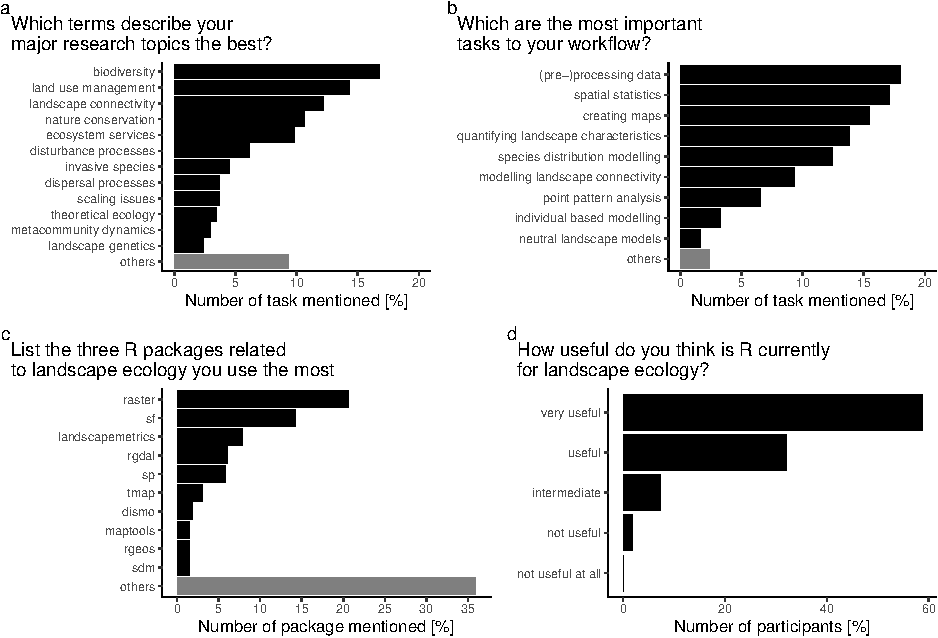
\includegraphics{paper_files/figure-latex/fig-survey-1} 

}

\caption{Results of the online survey about open-source software tools in R for landscape ecology. Results include A) which terms describe major reserach topics the best, B) the most important workflow task, C) the most used R packages and D) the overall usefulnes or R for landscape ecology. 'others' includes all answers with less than five total mentions.}\label{fig:fig-survey}
\end{figure}

\FloatBarrier

\hypertarget{missing-packages}{%
\section{Missing packages}\label{missing-packages}}

The survey also included a section in which participants could list methods and tools that are currently missing in \emph{R} and answers to this question were very diverse.
Overall, 21.9\% of the participants reported that currently no packages and functionality are missing for them or they lack the overview to answer the question.
There were two most common topics across the answers of the participants .
Firstly, many participants (13.5\%) wished for a better computational performance of \emph{R} in terms of speed and required RAM for larger data.
Secondly, many participants (9.4\%) are currently missing advanced and easy-to-apply methods for creating high-quality maps or other visualization-related functionality.
Fewer participants were missing tools for various connectivity-related issues (9.4\%) and characterization of landscape characteristics (7.3\%).

\bibliographystyle{spphys}
\bibliography{bibliography.bib}

\end{document}
